\section{Point Estimation}

  \begin{definition}[Sample Statistic, Estimators and Estimates]
    Now given a population $X$, we would like to use the $n$ iid samples $x_1, \ldots, x_n$ to estimate a parameter $\theta$ of interest with our own random variable/value $\widehat{\theta}_n$, called a \textbf{sample statistic}. We must note the dual nature of the sample statistic as a random variable and a value is similar to that of samples. 
    \begin{enumerate}
      \item The statistic $\widehat{\theta}_n$ is a random variable itself, referred to as the \textbf{estimator}. More specifically, it is a function $\widehat{\theta}_n: \mathbb{R}^n \longrightarrow \mathbb{R}$ of the $n$ samples, i.e. a transformation of random variables 
      \begin{equation}
        \widehat{\theta}_n = \widehat{\theta}_n (x_1, x_2, \ldots, x_n)
      \end{equation}
      This makes $\widehat{\theta}_n$ also a random variable, which attempts to estimate the true $\theta$, which is some unknown fixed value. Since $\widehat{\theta}_n$ is a random variable, it has its own distribution, called the \textbf{sampling distribution} of $\widehat{\theta}_n$. 
      
      \item Once these samples $x_i$ have been realized, the estimator realizes and the value realized is now called the \textbf{estimate}. 
    \end{enumerate}
    This sampling distribution is a distribution of the statistic $\widehat{\theta}_n$, and this forms a separate distribution with its own mean and variance. 
    \begin{enumerate}
      \item the mean of the sampling distribution is denoted $\mu_{\widehat{\theta}_n}$
      \item the standard deviation of the sampling distribution is denoted $\sigma^2_{\widehat{\theta}_n}$, also called the \textbf{standard error}. 
    \end{enumerate}
  \end{definition}

  We would want these estimators to have three properties: 
  \begin{enumerate}
    \item unbiasedness
    \item consistency 
    \item efficiency
  \end{enumerate}

  We would like the sampling distribution of our statistic to give us good estimate in two ways. $\widehat{\theta}_n$ should not be too far off from the actual parameter $\theta$ (bias is small), and $\widehat{\theta}_n$ should not fluctuate too widely (variance of $\widehat{\theta}_n$ should be small). 

  \begin{definition}[Bias, Variance of Estimator]
    Given an estimator $\widehat{\theta}$ of a sample $x_1, \ldots, x_n$ estimating population parameter $\theta$, the \textbf{sampling bias} refers to 
    \begin{equation}
      \mathrm{Bias}(\widehat{\theta}) = \big| \mathbb{E}[\widehat{\theta}] - \theta \big|
    \end{equation}
    and the \textbf{sampling variance} refers to 
    \begin{equation}
      \mathrm{Var}(\widehat{\theta}) = \mathbb{E} \big[ (\widehat{\theta} - \mathbb{E}[\widehat{\theta}])^2 \big]
    \end{equation}
  \end{definition}

  A good rule of thumb to remember is that statistics is about replacing expectations with averages. 
  \begin{equation}
    \mathbb{E} \mapsto \frac{1}{n} \sum_i
  \end{equation}
  This is really the fundamental quality of statistics. Then after that we can do some fancy things, like minimizing something or manipulating another, but every single time we see an expectation just replace it with an average. 

  \begin{definition}[Sample Mean]
    Given a population $X$ with $\mu = \mathbb{E}[X]$ and $\sigma^2 = \mathrm{Var}(X)$, our estimator for $\mu$ is simply the average of the $n$ samples $x_1, \ldots, x_n$, called the \textbf{sample mean} or the \textbf{sampling distribution of the sample mean}. 
    \begin{equation}
      \overline{x}_n = \widehat{\mu}_n = \frac{1}{n} (x_1 + \ldots + x_n)
    \end{equation}
    This gives us the sampling distribution of the sample means. The mean and standard deviation (i.e. standard error) of $\overline{x}_n$ is denoted $\mu_{\overline{x}_n}$ and $\sigma_{\overline{x}_n}$. 
    \begin{enumerate}
      \item The mean of $\overline{x}_n$ is $\mu$. 
      \begin{equation}
        \mu_{\overline{x}_n} = \mu
      \end{equation}
      because
      \begin{equation}
        \mathbb{E}[\overline{x}_n] = \mathbb{E} \bigg[ \frac{1}{n} \sum_{i=1}^n x_i \bigg] = \frac{1}{n} \sum_{i=1}^n \mathbb{E}[x_i] = \mathbb{E}[x] = \mu
      \end{equation}
      
      \item The variance of $\overline{x}_n$ is $\sigma^2 / n$, i.e. the standard error of $\overline{x}_n$ is $\sigma_{\overline{x}_n} = \sigma / \sqrt{n}$. 
      \begin{equation}
        \sigma_{\overline{x}_n} = \frac{\sigma}{\sqrt{n}}
      \end{equation}
      because 
      \begin{equation}
        \sigma^2_{\overline{x}_n} = \frac{1}{n^2} \sum_{i=1}^n \mathrm{Var}(x_i) = \frac{1}{n} \mathrm{Var}(x) = \frac{\sigma^2}{n}
      \end{equation}
       Practically, this tells us that when trying to estimate the value of a population mean, due to the factor of $1/\sqrt{n}$, reducing the error on the estimate by a factor of $2$ requires acquiring $4$ times as many observations in the sample. But realistically, the true standard deviation $\sigma$ is unknown, and so the standard error of the mean is usually estimated by replacing $\sigma$ with the sample standard deviation $S$ instead. 
      \begin{equation}
        \sigma_{\overline{x}_n} \approx \frac{S}{\sqrt{n}}
      \end{equation}

      \item By CLT, $\overline{x}_n$ converges to $\mathcal{N}(\mu, \sigma^2/n)$ in distribution as $n \rightarrow +\infty$ (but in practicality, we assume this for $n \geq 30$). The fact that its mean and variance is $\mu$ and $\sigma^2 /n$ isn't that impressive. What is really impressive is that no matter what the distribution of $x$ is, the sampling distribution of the mean will be Gaussian. 
    \end{enumerate}
  \end{definition}

  \begin{example}[Sample Means]
    Here are some figures of sample means. Note that with a uniform parent distribution, the sampling distribution of its mean looks like a Gaussian even without a large $n$. However, this is not necessarily true for different parent distributions, such as the exponential. 
    \begin{figure}[H]
      \centering
      \begin{subfigure}[b]{0.48\textwidth}
      \centering
        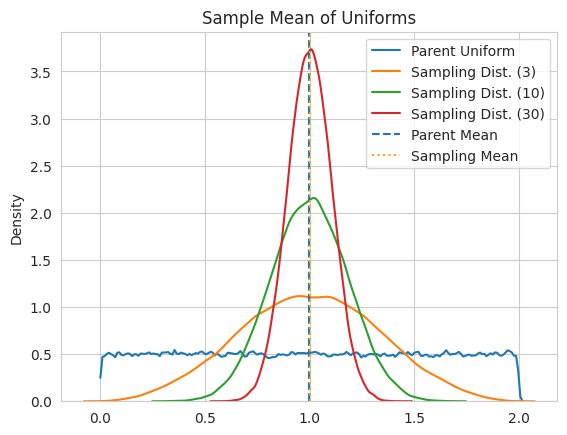
\includegraphics[width=\textwidth]{img/sample_mean_uniform.png}
        \caption{We plot the PDF of an $X \sim \mathrm{Uniform}[0, 2]$ random variable by taking 100k samples. We also take 100k samples from the sampling distribution of the mean $\overline{X}_{3}, \overline{X}_{10}, \overline{X}_{30}$. We can see that the standard deviation decreases by a factor of $\sqrt{n}$.}
        \label{fig:sample_mean_uniform}
      \end{subfigure}
      \hfill 
      \begin{subfigure}[b]{0.48\textwidth}
      \centering
        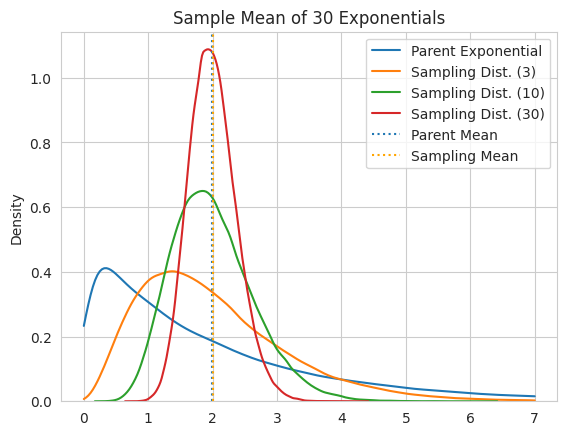
\includegraphics[width=\textwidth]{img/sample_mean_exp.png}
        \caption{We plot the PDF of an $X \sim \mathrm{Exponential}(1.5)$ random variable by taking 100k samples. We also take 100k samples from the sampling distribution of the mean $\overline{X}_{3}, \overline{X}_{10}, \overline{X}_{30}$. }
        \label{fig:sample_mean_exp}
      \end{subfigure}
      \caption{}
      \label{fig:sample_mean_examples}
    \end{figure}
  \end{example}

  If the parent distribution is normal, then we don't even need CLT to claim that the sampling distribution of the sample mean is normal, since sums of normals are normal. 

  Now the variance of the population is defined to be $\sigma^2 = \mathbb{E}[ (X - \mathbb{E}[X])^2 ]$, and by our rule of thumb, we can replace the expectations with sample means, by first setting $\mathbb{E}[X] = \widehat{\mu}$ and averaging out the values $(X - \widehat{\mu})^2$. 

  \begin{definition}[Sample Variance]
    Given a population $X$, our estimator for $\sigma^2 = \mathbb{E}[ (X - \mathbb{E}[X])^2 ]$ is simply the average of the squared distances of the $n$ samples $\{(x_i - \widehat{\mu})^2\}_{i=1}^n$. 
    \begin{equation}
      S^2_n = \widehat{\sigma}^2_n = \frac{1}{n} \sum_{i=1}^n ( x_i - \overline{x}_n)^2
    \end{equation}
    The mean and standard deviation of $S^2_n$ is denoted $\mu_{S^2_n}$ and $\sigma_{S^2_n}$. Note that there is a small difference that the sum for variance is divided by $n-1$ rather than $n$, since we want it to be unbiased, but we will correct this later. 
  \end{definition}

  While the CLT states that the sampling distribution of the sample mean will look approximately Gaussian, we do not have this luxury when looking at the sampling distribution of sample variance. 

  \begin{example}[Sample Variance]
    Take a look at the following sampling distributions of the sample variance. There does not seem to be strong signs of convergence to a Gaussian. Their means do not align either. 
    \begin{figure}[H]
      \centering
      \begin{subfigure}[b]{0.48\textwidth}
      \centering
        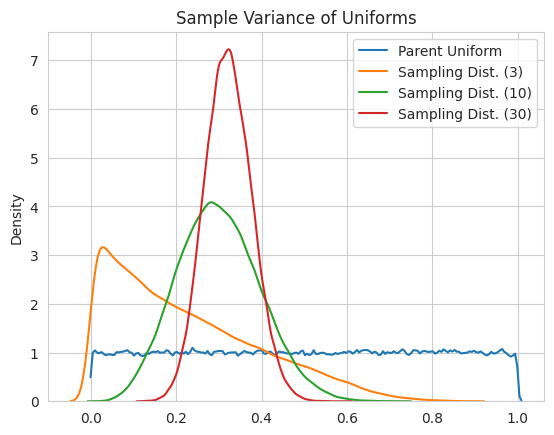
\includegraphics[width=\textwidth]{img/sample_variance_uniform.png}
        \caption{}
        \label{fig:sample_variance_uniform}
      \end{subfigure}
      \hfill 
      \begin{subfigure}[b]{0.48\textwidth}
      \centering
        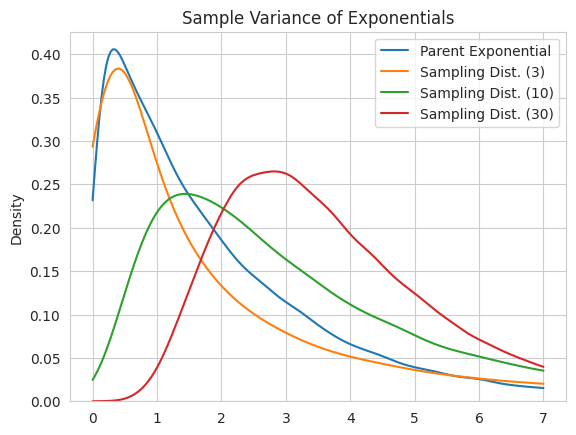
\includegraphics[width=\textwidth]{img/sample_variance_exp.png}
        \caption{}
        \label{fig:sample_variance_exp}
      \end{subfigure}
      \caption{}
      \label{fig:sample_variance_examples}
    \end{figure}
  \end{example}

\subsection{Sampling from Gaussians}

  Now if we assume that the parent distribution is Gaussian, then we can conclude some extra things and more kinds of distributions arise. Let $x_1, \ldots, x_n \sim \mathcal{N}(\mu, \sigma^2)$, with $\overline{x}_n$ the sample mean and $S^2_n$ the sample variance. Say that we want to find the distribution of $\overline{x}_n$. 
  \begin{enumerate}
    \item In the unrealistic case where we know the true $\sigma^2$, we don't even need to consider the sample variance. From the basic property of Gaussians, we know that $\overline{x}_n \sim \mathcal{N}(\mu, \sigma^2/n)$, or after standardizing, 
    \begin{equation}
      \frac{\overline{x}_n - \mu}{\sigma/\sqrt{n}} \sim \mathcal{N}(0, 1)
    \end{equation}
    \item In the realistic case where we don't know the true $\sigma^2$, we should replace it with our sample variance $S^2$, and it turns out that because of this extra uncertainty in the variance, our sampling distribution follows the student-t distribution, which can be interpreted as a mixture of Gaussians with differing variances. 
    \begin{equation}
      \frac{\overline{x}_n - \mu}{S/\sqrt{n}} \sim \mathrm{StudentT}(n-1)
    \end{equation}
  \end{enumerate}
  Now if we are interested in finding the distribution of $S^2_n$: 
  \begin{enumerate}
    \item In the unrealistic case where the know the true $\mu$, we don't need to consider the sampling distribution of $\overline{x}_n$. We have 
    \begin{equation}
      S^2_n = \frac{1}{n} \sum_{i=1}^n (x_i - \mu)^2 \sim \mathrm{Gamma}\Big( \frac{n}{2}, \frac{n}{2 \sigma^2} \Big)
    \end{equation}
    \item In the realistic case where we don't know $\mu$, we have 
    \begin{equation}
      \frac{n-1}{\sigma^2} S^2_n = \frac{1}{\sigma^2} \sum_{i=1}^n (x_i - \overline{x}_n )^2 \sim \chi^2 (n-1)
    \end{equation}
  \end{enumerate}

\subsection{Bias Variance Noise Decomposition} 

  Let's do some further analysis on this. When you take a supremum over a function class, it decomposes into 3 terms. 
  \begin{enumerate}
    \item One of which quantifies how big the function class is (more variance). 
    \item One of which quantifies the distance between the truth and the function class (bias).  
    \item One is the noise term, which is the irreducible error. 
  \end{enumerate}

  \begin{example}[Bias and Variance Tradeoff in Polynomial Regression]
    Let's motivate this by trying to fit a polynomial on some data. 
    \begin{figure}[H]
      \centering 
      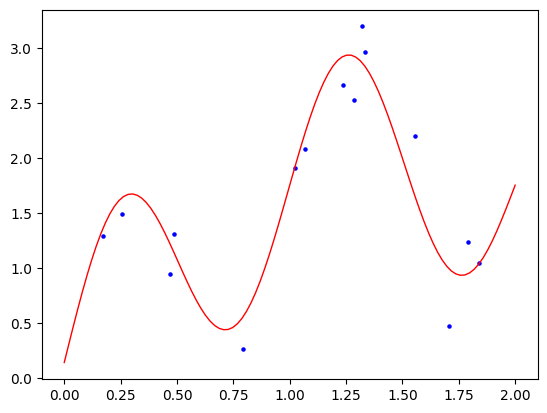
\includegraphics[scale=0.4]{img/True_data.png}
      \caption{A sample of $|\mathcal{D}| = 15$ data points are generated from the function $f(x) = \sin(2\pi x) + 2\cos (x - 1.5)$ with Gaussian noise $N(0, 0.3)$ on the interval $[0, 1]$. } 
      \label{fig:true_data}
    \end{figure}

    If we try to fit a polynomial function, how do we know which degree is best? Well the most simple thing is to just try all of them. To demonstrate this even further, I generated 10 different datasets  $\mathcal{D}$ of size $15$ taken from the same true distribution. The best fitted polynomials for each dataset is shown below. 

    \begin{figure}[H]
      \centering 
      \begin{subfigure}[b]{0.32\textwidth}
      \centering
        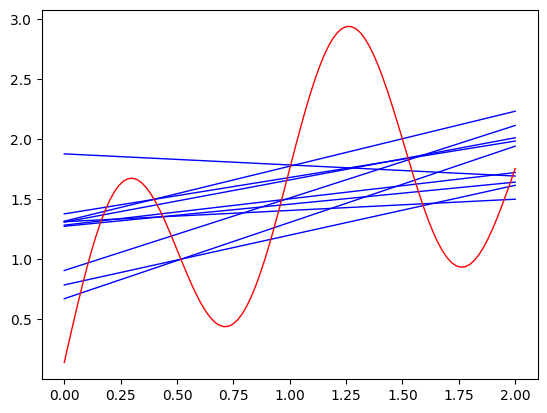
\includegraphics[width=\textwidth]{img/poly_1_fit.png}
        \caption{1st Degree}
        \label{fig:1d}
      \end{subfigure}
      \hfill 
      \begin{subfigure}[b]{0.32\textwidth}
      \centering
        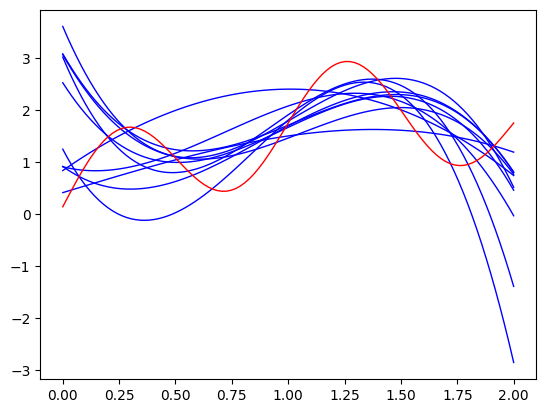
\includegraphics[width=\textwidth]{img/poly_3_fit.png}
        \caption{3rd Degree}
        \label{fig:3d}
      \end{subfigure}
      \hfill 
      \begin{subfigure}[b]{0.32\textwidth}
      \centering
        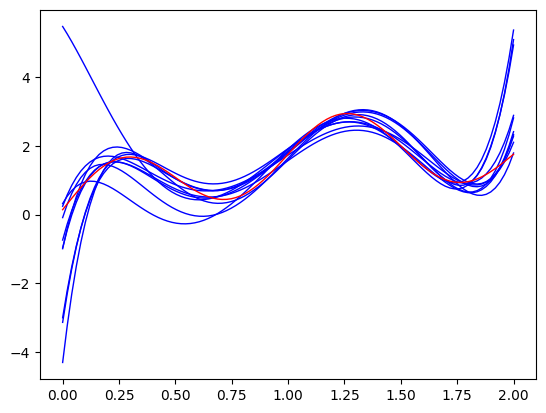
\includegraphics[width=\textwidth]{img/poly_5_fit.png}
        \caption{5th Degree}
        \label{fig:5e}
      \end{subfigure}

      \begin{subfigure}[b]{0.32\textwidth}
      \centering
        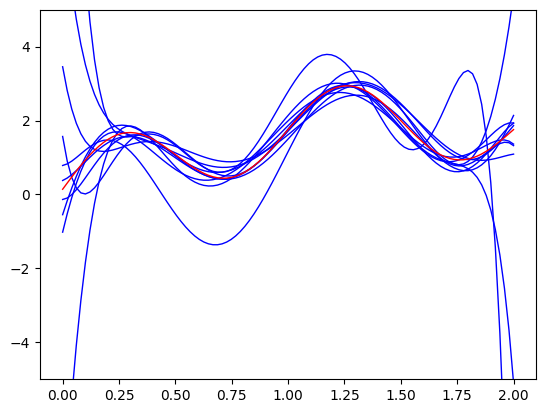
\includegraphics[width=\textwidth]{img/poly_7_fit.png}
        \caption{7th Degree}
        \label{fig:7d}
      \end{subfigure}
      \hfill 
      \begin{subfigure}[b]{0.32\textwidth}
      \centering
        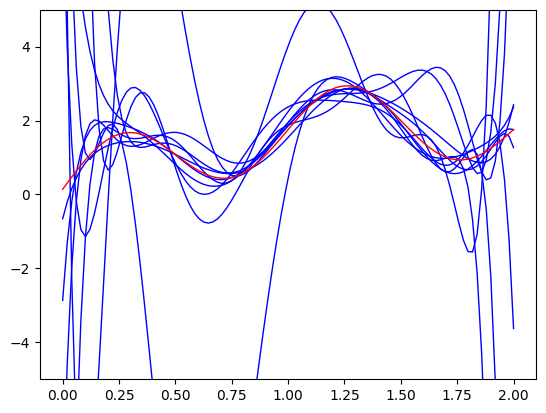
\includegraphics[width=\textwidth]{img/poly_9_fit.png}
        \caption{9th Degree}
        \label{fig:9d}
      \end{subfigure}
      \hfill 
      \begin{subfigure}[b]{0.32\textwidth}
      \centering
        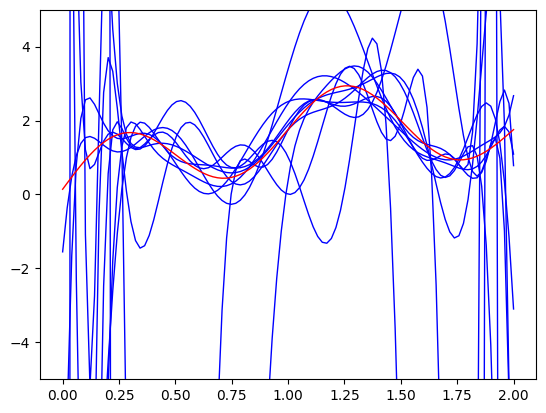
\includegraphics[width=\textwidth]{img/poly_11_fit.png}
        \caption{11th Degree}
        \label{fig:11e}
      \end{subfigure}

      \caption{Different model complexities (i.e. different polynomial degrees) lead to different fits of the data generated from the true distribution. The lower degree best fit polynomials don't have much variability in their best fits but have high bias, while the higher degree best fit polynomials have very high variability in their best fits but have low bias. The code used to generate this data is \href{code/polynomial_fitting.ipynb}{here}. }
      \label{fig:polynomial_fitting}
    \end{figure}

    We already know that the 5th degree approximation is most optimal, and the lower degree ones are \textbf{underfitting} the data, while the higher degree ones are \textbf{overfitting}. As mentioned before, we can describe the underfitting and overfitting phenomena through the bias variance decomposition. 

    \begin{enumerate}
      \item If we underfit the data, this means that our model is not robust and does not capture the patterns inherent in the data. It has a high bias since the set of function it encapsulates is not large enough to model $\mathbb{E}[Y\mid X]$. However, it has a low variance since if we were to take different samples of the dataset $\mathcal{D}$, the optimal parameters would not fluctuate. 

      \item What overfitting essentially means is that our model is too complex to the point where it starts to fit to the \textit{noise} of the data. This means that the variance is high, since different samples of the dataset $\mathcal{D}$ would cause huge fluctuations in the optimal trained parameters $\boldsymbol{\theta}$. However, the function set would be large, and thus it would be close to $\mathbb{E}[Y \mid X]$, leading to a low bias. 
    \end{enumerate}
  \end{example}
  
  \begin{example}[Polynomial Regression Continued]
    Another way to reduce the overfitting problem is if we have more training data to work with. That is, if we were to fit a 9th degree polynomial on a training set of not $N = 15$, but $N = 100$ data points, then we can see that this gives a much better fit. This makes sense because now the random variable $\mathcal{D}$, as a function of more random variables, has lower variance. Therefore, the lower variance in the dataset translates to lower variance in the optimal parameter. 

    \begin{figure}[H]
      \centering
      \begin{subfigure}[b]{0.48\textwidth}
      \centering
        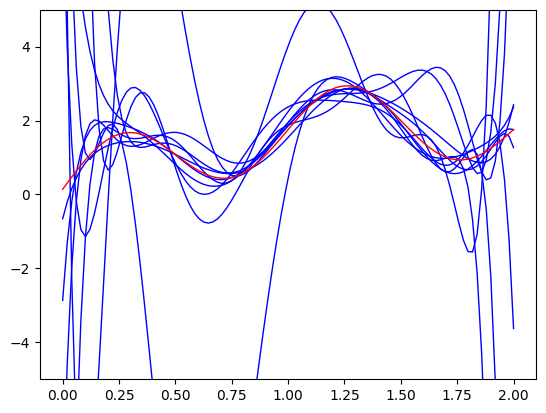
\includegraphics[width=\textwidth]{img/poly_9_fit.png}
        \caption{$M = 9, N = 15$}
        \label{fig:less_points}
      \end{subfigure}
      \hfill 
      \begin{subfigure}[b]{0.48\textwidth}
      \centering
        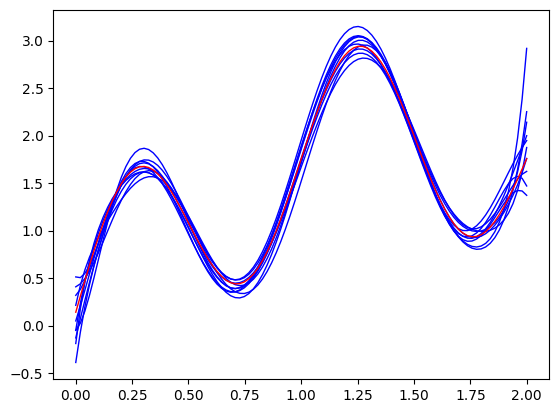
\includegraphics[width=\textwidth]{img/increased_data.png}
        \caption{$M = 9, N = 100$}
        \label{fig:more_points}
      \end{subfigure}
      \caption{Increasing the number of data points helps the overfitting problem. Now, we can afford to fit a 9th degree polynomial with reasonable accuracy.}
      \label{fig:reducing_overfitting_with_more_samples}
    \end{figure}
  \end{example}

